
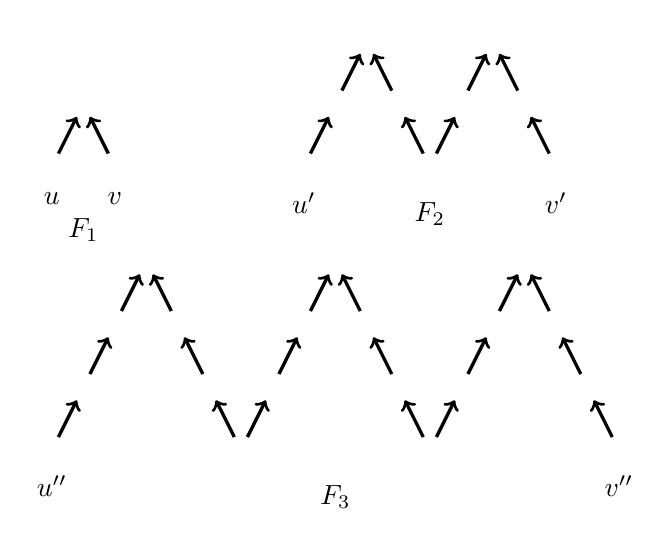
\begin{tikzpicture}[
    scale=0.4,
    line width=1.2pt
]

    \node at (-3,-6) {\(F_1\)};
    
    \node[circle, , label=below:{\(u\)}]
            (p0) at (-4,-4) {};

    \node[circle, , label=below:{\(v\)}]
            (p1) at (-2,-4) {};

    \node[circle, ]
        (p2) at (-3,-2) {};
    

    \draw[->] (p0) -- (p2);
    \draw[->] (p1) -- (p2);

    \onslide<2->{
    \node at (8,-5.5) {\(F_2\)};
            
    \node[circle, , label=below:{\(u'\)}]
            (q0) at (4,-4) {};
    \node[circle, , label=below:{}]
            (q1) at (8,-4) {};
    \node[circle, , label=below:{\(v'\)}]
            (q2) at (12,-4) {};
    \node[circle, , label=below:{}]
            (q3) at (5,-2) {};
    \node[circle, , label=below:{}]
            (q4) at (7,-2) {};
    \node[circle, , label=below:{}]
            (q5) at (9,-2) {};
    \node[circle, , label=below:{}]
            (q6) at (11,-2) {};
    \node[circle, , label=below:{}]
        (q7) at (6,0) {};
    \node[circle, , label=below:{}]
        (q8) at (10,0) {};   
        
    \draw[->] (q0) -- (q3);
    \draw[->] (q3) -- (q7);
    \draw[->] (q4) -- (q7);
    \draw[->] (q1) -- (q4);
    \draw[->] (q1) -- (q5);
    \draw[->] (q2) -- (q6);
    \draw[->] (q5) -- (q8);
    \draw[->] (q6) -- (q8);
    }

    \onslide<3>{
    \node at (5,-14.5) {\(F_3\)};
            
    \node[circle, , label=below:{\(u''\)}]
            (r0) at (-4,-13) {};
    \node[circle, , label=below:{}]
            (r1) at (2,-13) {};
    \node[circle, , label=below:{}]
            (r2) at (8,-13) {};
    \node[circle, , label=below:{\(v''\)}]
            (r3) at (14,-13) {};
    \node[circle, , label=below:{}]
            (r4) at (-3,-11) {};
    \node[circle, , label=below:{}]
            (r5) at (1,-11) {};
    \node[circle, , label=below:{}]
            (r6) at (3,-11) {};
    \node[circle, , label=below:{}]
            (r7) at (7,-11) {};
    \node[circle, , label=below:{}]
            (r8) at (9,-11) {};
    \node[circle, , label=below:{}]
            (r9) at (13,-11) {};
    \node[circle, , label=below:{}]
            (r10) at (3,-11) {};
    \node[circle, , label=below:{}]
            (r11) at (-2,-9) {};
    \node[circle, , label=below:{}]
            (r12) at (0,-9) {};
    \node[circle, , label=below:{}]
            (r13) at (4,-9) {};
    \node[circle, , label=below:{}]
            (r14) at (6,-9) {};
    \node[circle, , label=below:{}]
            (r15) at (10,-9) {};
    \node[circle, , label=below:{}]
            (r16) at (12,-9) {};
    \node[circle, , label=below:{}]
            (r17) at (-1,-7) {};
    \node[circle, , label=below:{}]
            (r18) at (5,-7) {};
    \node[circle, , label=below:{}]
            (r19) at (11,-7) {};

    \draw[->] (r0) -- (r4);
    \draw[->] (r1) -- (r5);
    \draw[->] (r1) -- (r6);
    \draw[->] (r2) -- (r7);
    \draw[->] (r2) -- (r8);
    \draw[->] (r3) -- (r9);
    \draw[->] (r4) -- (r11);
    \draw[->] (r5) -- (r12);
    \draw[->] (r6) -- (r13);
    \draw[->] (r7) -- (r14);
    \draw[->] (r8) -- (r15);
    \draw[->] (r9) -- (r16);
    \draw[->] (r11) -- (r17);
    \draw[->] (r12) -- (r17);
    \draw[->] (r13) -- (r18);
    \draw[->] (r14) -- (r18);
    \draw[->] (r15) -- (r19);
    \draw[->] (r16) -- (r19);
    
        
    }



    
\end{tikzpicture}
